\fancyfoot[RE,LO]{Autor: Claudia Fuchs}

\section {EOG} \label {eog}

\subsection {Einleitung} \label {eog einleitung}

Die Elektrookulografie ist ein Messverfahren, womit Augenbewegungen gemessen werden k"onnen. Die Messung basiert dabei auf der Potentialdifferenz zwischen der vorne gelegenen, positiv geladenen Cornea (Hornhaut) und der hinten gelegenen negativ geladenen Retina (Netzhaut). Das Auge kann also als Dipol betrachtet werden, dessen Spannung sich bei Bewegungen des Auges ver"andert. Diese Ver"anderung kann mittels Oberfl"achenelektroden in Augenn"ahe gemessen und in einem Elektrookulogramm dargestellt werden. \cite{reg205}

\begin{figure}[h]
	\centering
		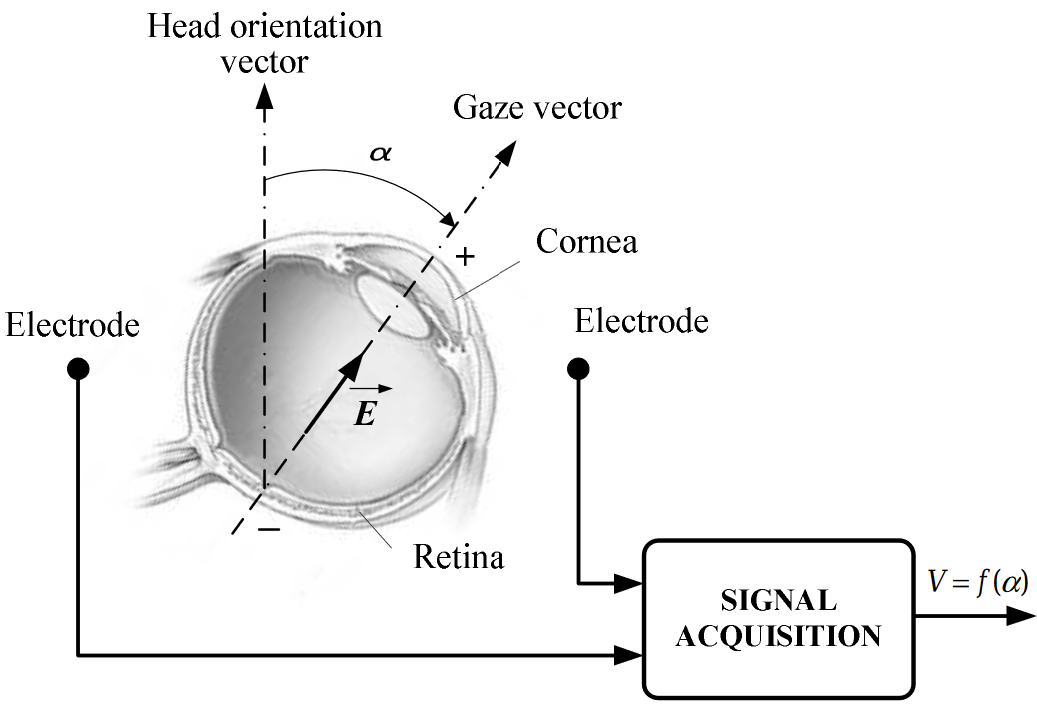
\includegraphics[width=0.9\textwidth]{Fuchs/Augendipol.png}
	\caption{Veranschaulichung des Augendipols durch Potentialdifferenz von Retina und Cornea}
	\label{fig:Augendipol}
\end{figure}

Abbildung \ref{fig:Augendipol} bildet den Blickvektor sowie dessen Ver"anderungspotential ab.  Eine Augenbewegung um $\alpha$ kann "uber die Elektroden gemessen und das Signal durch eine entsprechende Messschaltung aufbereitet werden. \cite{reg205}\\
Im Rahmen unseres Diplomprojekts soll es aber vorallem um die Schlafanalyse gehen. Wie bereits im Kapitel \ref{schlaf} er"ortert, zeichnet sich die REM-Schlafphase durch schnelle Augenbewegungen aus. Diese gilt es mittels EOG-Schaltung als solche zu erkennen. 

\subsubsection {Signalparameter} \label {signalparamater}

Bevor eine Messschaltung entwickelt werden kann ist es wichtig, die Signalparamter wie Amplitude und Bandbreite des zu messenden Biosignals in Erfahrung zu bringen.\\
Im Falle des EOGs ist die Amplitude typischerweise zwischen 0.05 und 3.5mV je nach Umgebung, Elektrodenplatzierung und St"arke der Augenbewegung. Die Bandbreite reicht von 0 bis 50Hz, wobei die meiste Information des Signals zwischen 0.1 und zirka 40Hz steckt. \cite{reg205},\cite{reg203}

INA-Testmessung
\subsubsection {Elektroden} \label {elektroden} 
Es gibt mehrere M"oglichkeiten, die Elektroden zur EOG-Messung im Gesicht anzubringen. Diese Unterscheiden sich sowohl in Position und Anzahl der Elektroden sowie der daraus resultierenden Genauigkeit der Messung.
\begin{figure}[h]
	\centering
		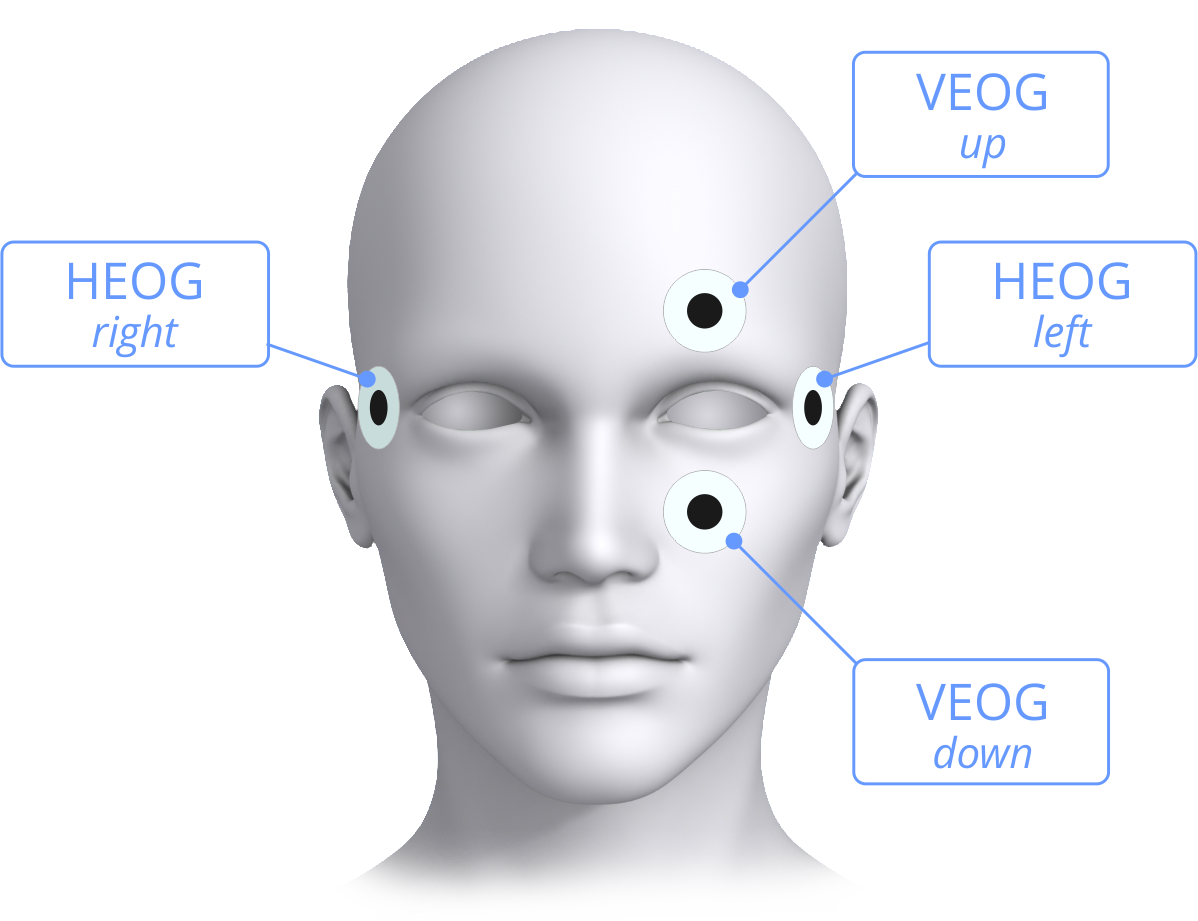
\includegraphics[width=0.9\textwidth]{Fuchs/Elektrodenplatzierung.png}
	\caption{Elektrodenplatzierung zur Messung horizontaler und vertikaler Augenbewegungen}
	\label{fig:Elektrodenplatzierung}
\end{figure}
F"ur unser Diplomprojekt wurde eine Methode mit 4 Elektroden gew"ahlt, welche in Abbildung \ref{fig:Elektrodenplatzierung} dargestellt wird. Zur Messung der vertikalen Augenbewegungen dienen dazu die "uber und unter dem Augen liegenden Elektroden, die Messung der horizontalen Augenbewegung erfolgt "uber die links und rechts angebrachten Elektroden. \\
Es handelt sich hierbei um Ag/AgCl-Oberfl"achenelektroden, welche auch bei EKG-Messungen verwendet werden k"onnen. 
\subsection {Signalflussdiagramm} \label {signalfluss}
\begin{figure}[H]
	\centering
		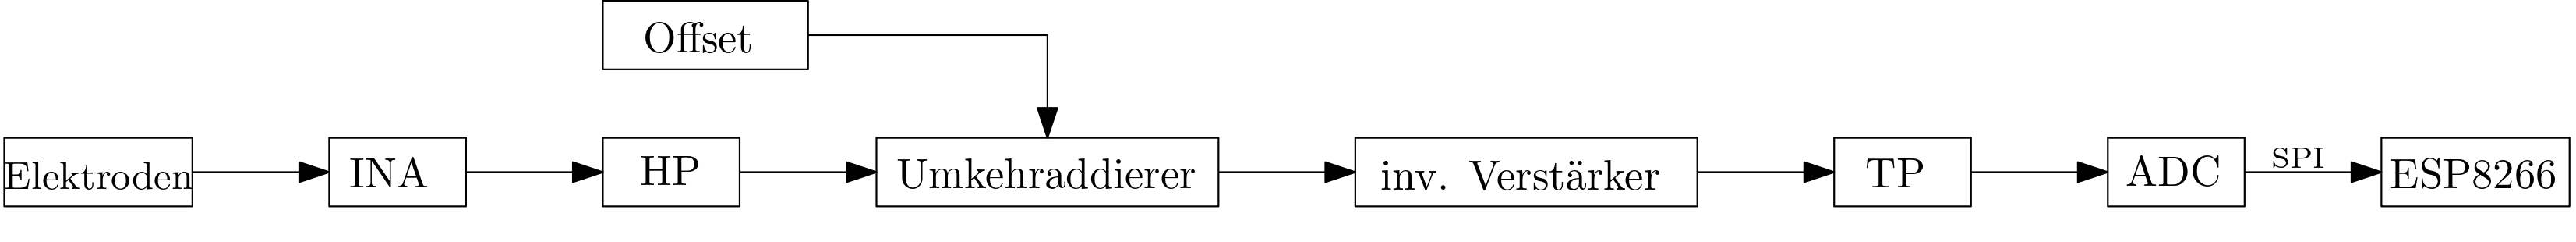
\includegraphics[width=0.9\textwidth]{Fuchs/Signalfluss.png}
	\caption{Signalflussdiagramm des EOGs.}
	\label{fig:signalfluss}
\end{figure}

In Abbildung \ref{fig:signalfluss} werden die einzelnen Bestandteile, die fu"r die Messung der Augenbewegungen ben"otigt werden, in einem Signalflussdiagramm dargestellt. Der genaue Aufbau dieser und die Dimensionierung der dazugeh"origen Bauteile werden in den n"achsten Abschnitten erl"autert. Es ist zus"atzlich anzumerken, dass es sich hierbei lediglich um die Messschaltung von einer Richtung (vertikal oder horizontal) handelt. Die Gesamtschaltung besteht demnach aus zwei identen Schaltungen, die sich einen ADC und Mikrocontroller teilen. 

\subsection {Filter} \label {filter}
Wie bereits im Kapitel \ref{signalparamater} erw"ahnt, betr"agt die f"ur uns relevante Bandbreite 0.1-40Hz. Wir ben"otigen also einen Hochpass, um die Gleichspannungskomponenten herauszufiltern und einen Tiefpass, der Frequenzen "uber 50Hz d"ampft und zugleich als Anti-Aliasingfilter f"ur den Analog-Digital-Wandler dient.\\
Es wurden dazu aktive Filter des Sallen-Key-Typs ausgew"ahlt und dimensioniert.

\subsubsection {Hochpass (2. Ordnung)} \label{hp}
\begin{figure}[H]
	\centering
		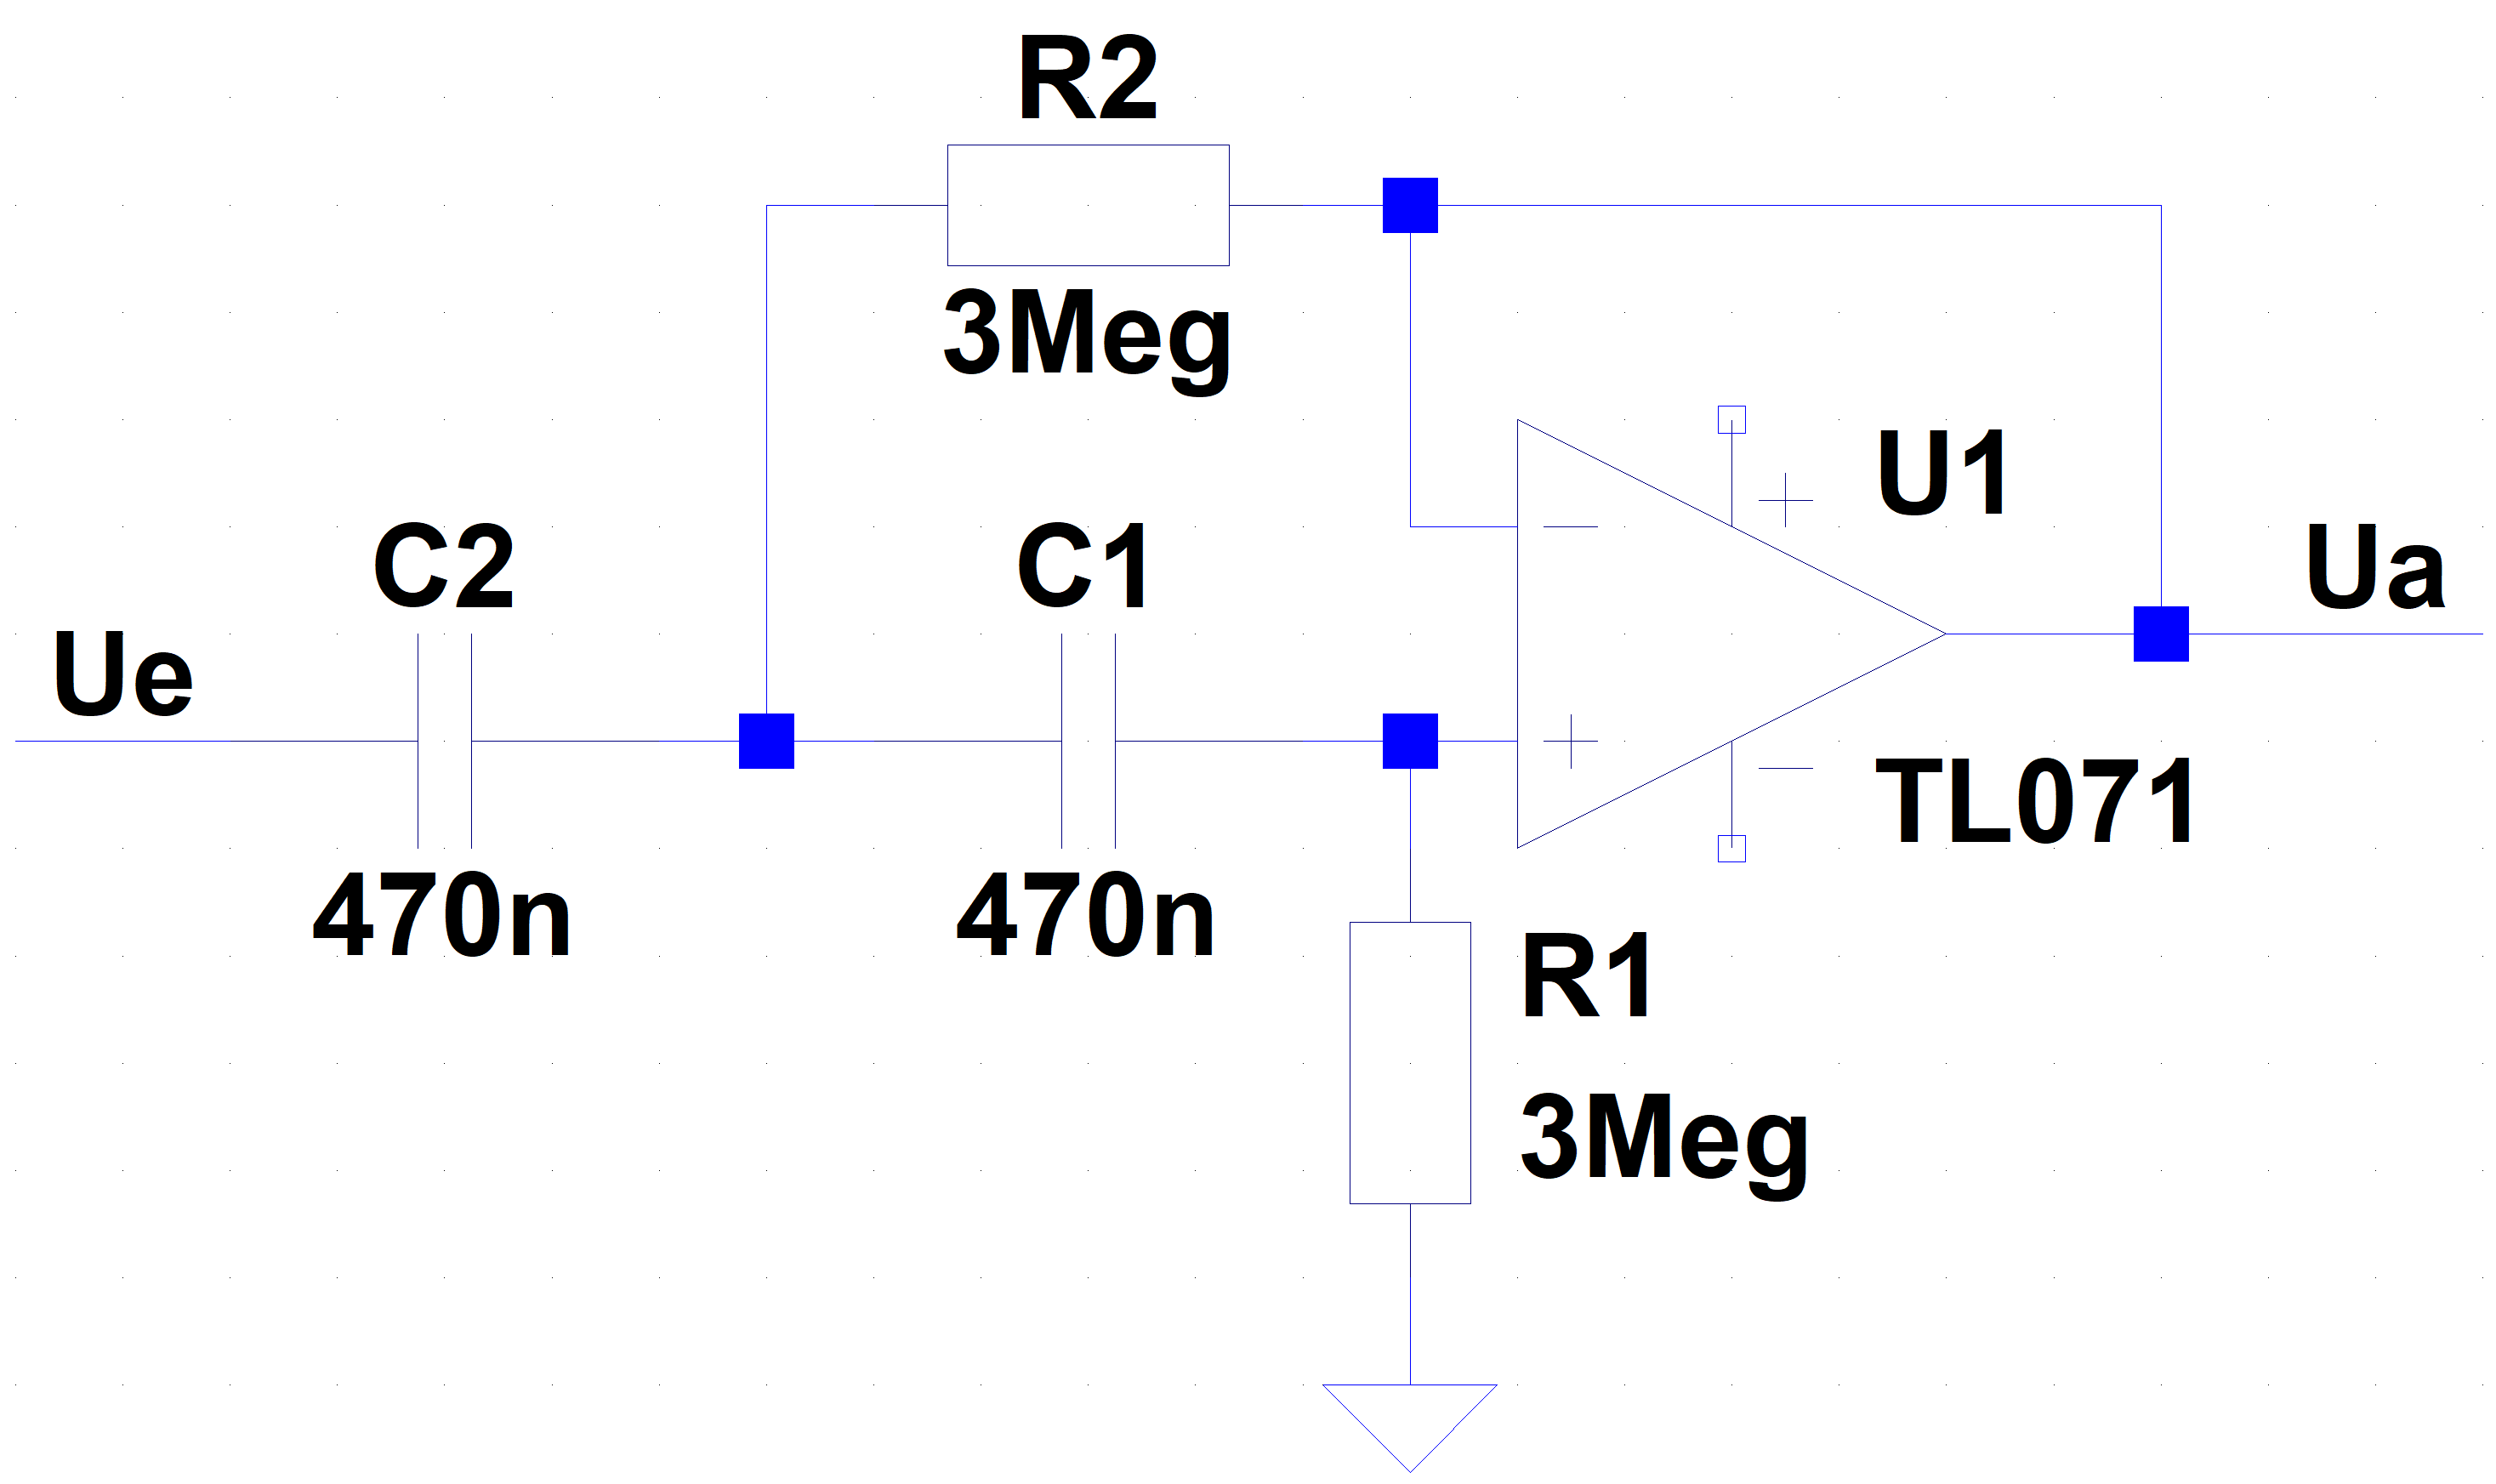
\includegraphics[width=0.9\textwidth]{Fuchs/Hochpass.png}
	\caption{OPV-Schaltung eines Hochpasses 2.Ordnung}
	\label{fig:hp}
\end{figure}

Zur Filterung des Gleichspannungsanteils wurde eine Schaltung, wie in Abbildung \ref{fig:hp} gezeigt, dimensioniert. Es handelt sich dabei um einen Hochpass zweiter Ordnung mit einer Grenzfrequenz $f_g = 0.11Hz$.

\subsubsection {Anti-Aliasing-/Tiefpassfilter (3.Ordnung)} \label{tp}
\begin{figure}[H]
	\centering
		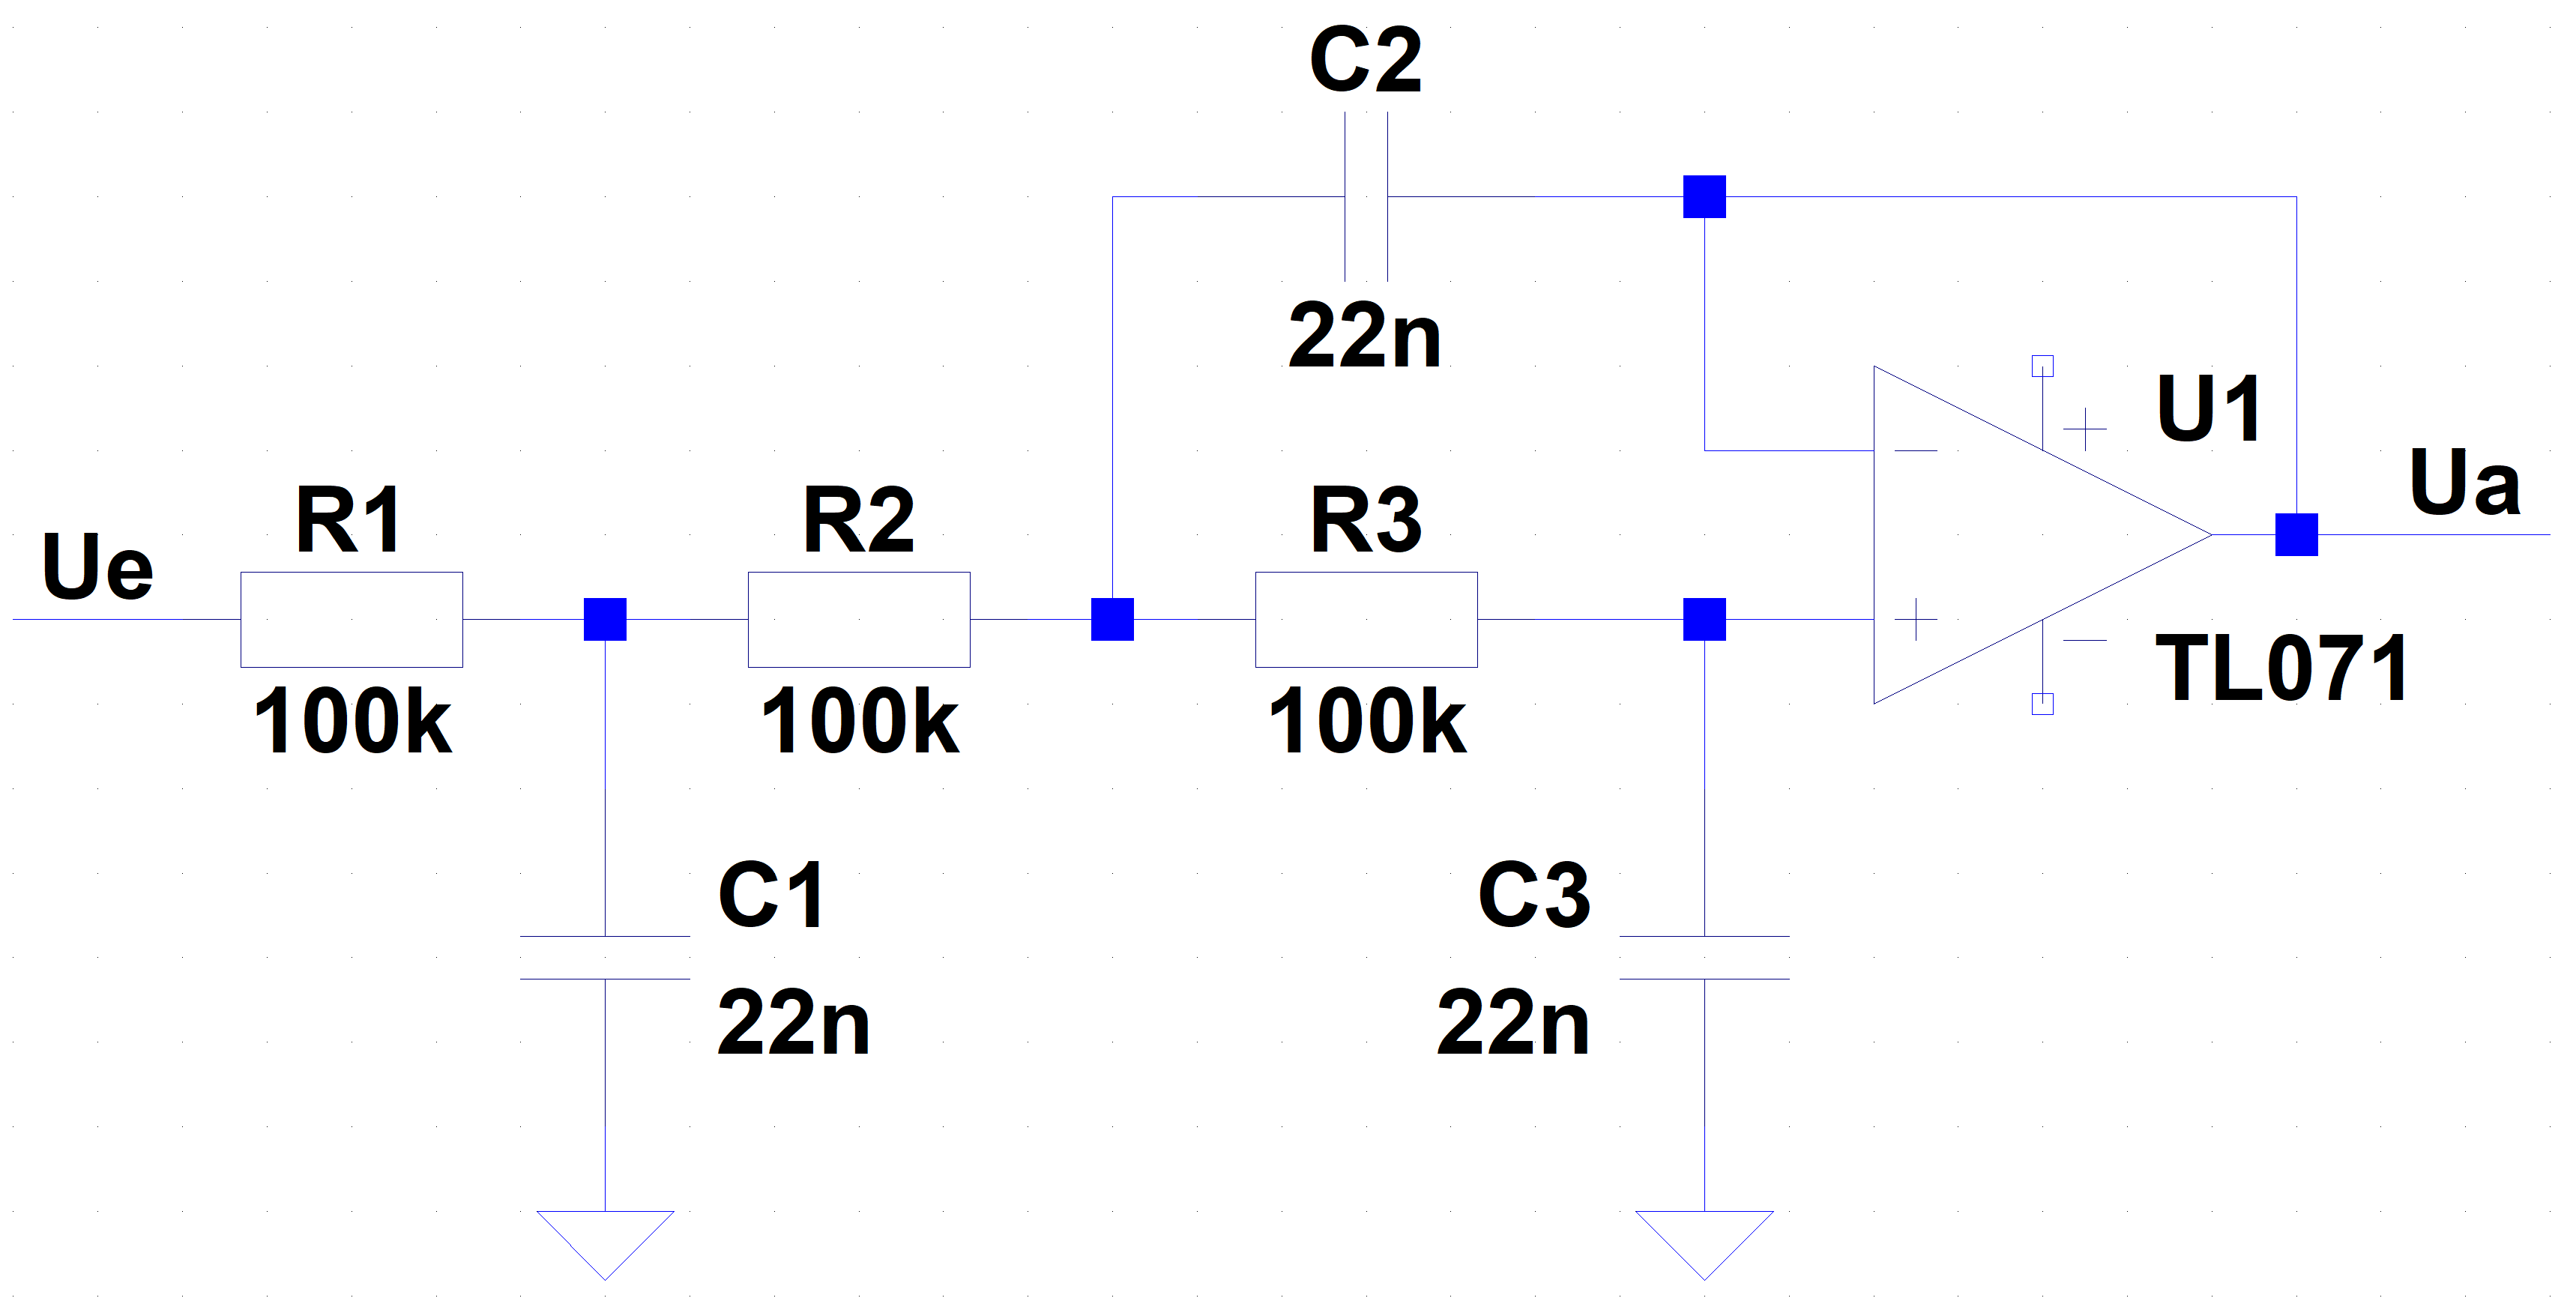
\includegraphics[width=0.9\textwidth]{Fuchs/Tiefpass.png}
	\caption{OPV-Schaltung eines Tiefpasses 3.Ordnung}
	\label{fig:tp}
\end{figure}

Zur D"ampfung h"oherer Frequenzen, die nicht zu unserem Nutzsignal geh"oren, wurde ein Tiefpass 3.Ordnung, wie in Abbildung \ref{fig:tp} gezeigt, dimensioniert. Die Grenzfrequenz betr"agt $f_g = 72Hz$\footnote{Die Bandbreite des Nutzsignals endet bereits bei ~40Hz. Die h"oher gew"ahlte Grenzfrequenz ist mit der Ordnung des Filters begr"undet, bei dessen Grenzfrequenz bereit -12dB des Signals ged"ampft werden, die eigentliche Grenzfrequenz (bei einer D"ampfung von -3dB) liegt also tiefer.}.

Welche Art von Filter, Bauteilwerte

\subsection {Verst"arkung} \label {verstaerkung}

Wie bereits im Kapitel \ref{signalparamater} erw"ahnt, handelt es sich beim EOG-Signal, wie bei den meisten Biosignalen, um eher kleinere Amplituden (0.05-3.5mV). Diese gilt es erst einmal messtechnisch zu verst"arken, um brauchbare Ergebnisse zu erhalten.

\subsubsection {Instrumentenverst"arker} \label{ina}
Der Instrumentenverst"arker verst"arkt die Differenz zwischen den beiden Eingangsspannungen. In unserem Fall die Differenz zwischen zwei Elektroden ("uber/unter dem Auge bzw. links und rechts der Augen). Die Verst"arkungsformel zur Dimensionierung f"ur den INA128 kann aus dem Datenblatt abgelesen werden und lautet:\\
\begin{equation}\label{eq:ina}
	G = 1 + {50k\Omega}/{R_G}
\end{equation}

Der Einfachkeit halber wurde $R_G$ zun"achst mit $1k\Omega$ angenommen. Daraus ergibt sich eine Verst"arkung von 51.

\paragraph {Testmessung der Rohdaten} \label {Rohdaten}
\textbf{\\Messschatltung:}
\begin{figure}[H]
	\centering
		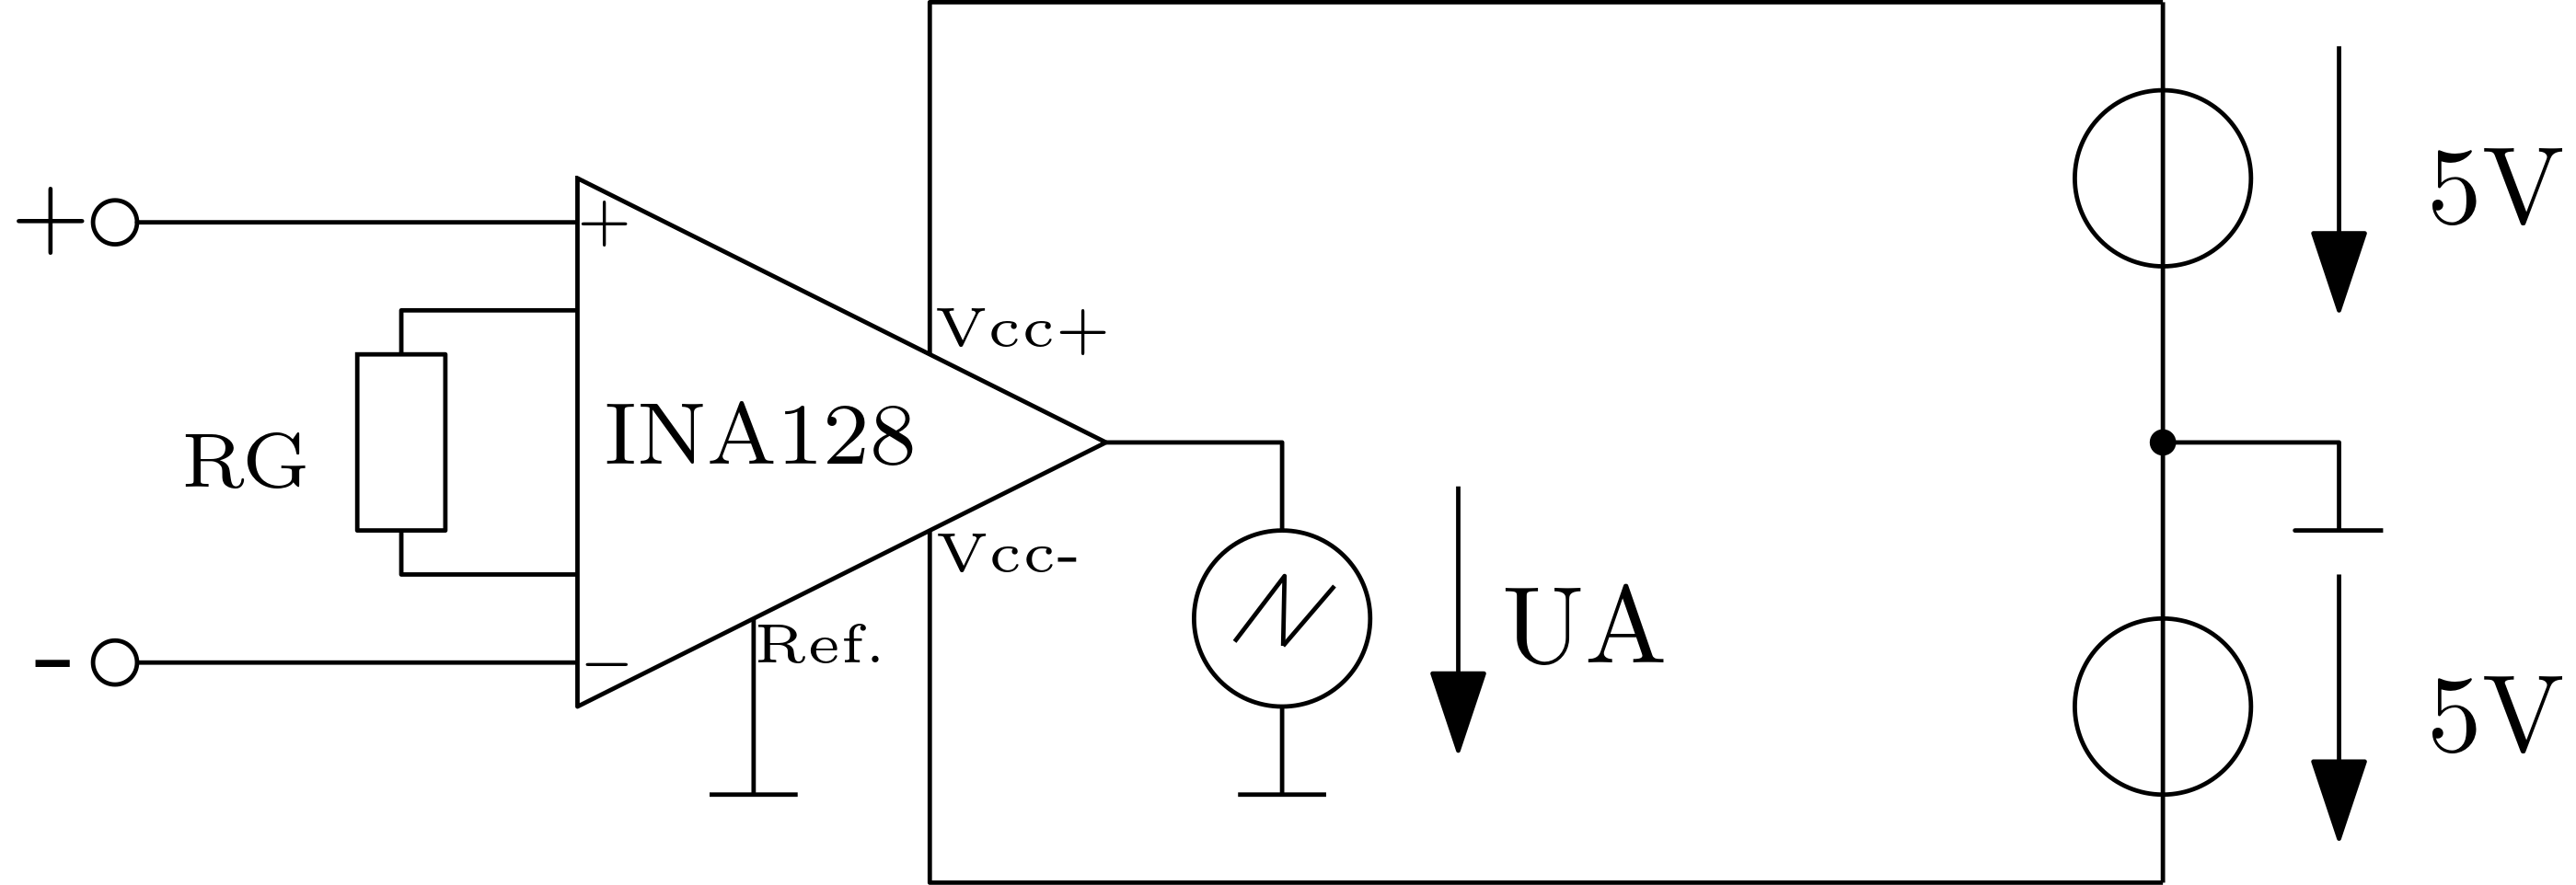
\includegraphics[width=0.9\textwidth]{Fuchs/Messschaltung-Rohdaten.png}
	\caption{Schaltung zur Messung der Rohdaten}
	\label{fig:ms_rohdaten}
\end{figure}

Der Verst"arkungswiderstand $R_G$ der in Abbildung \ref{fig:ms_rohdaten} dargestellt ist, entspricht $1k\Omega$ wie bei Gleichung \ref{eq:ina} berechnet. Die Versorgungsspannung mit $\pm5V$ sowie das Oszilloskop selbst sind Funktionen des AnalogDiscovery, einem portablen Oszilloskop, welche in Kapitel \ref{analogdiscovery} n"aher beschrieben werden. \\

\textbf{Messergebnisse:}
\begin{figure}[H]
	\centering
		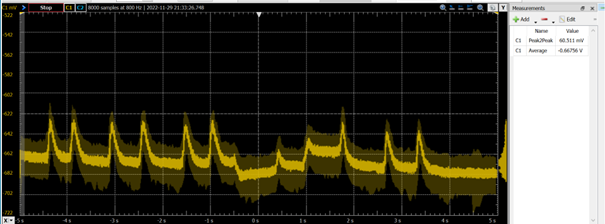
\includegraphics[width=0.9\textwidth]{Fuchs/Messergebnis_RohdatenV.png}
	\caption{Messung der Rohdaten von Augenbewegungen in vertikaler Richtung}
	\label{fig:me_rohdatenV}
\end{figure}
\begin{figure}[H]
	\centering
		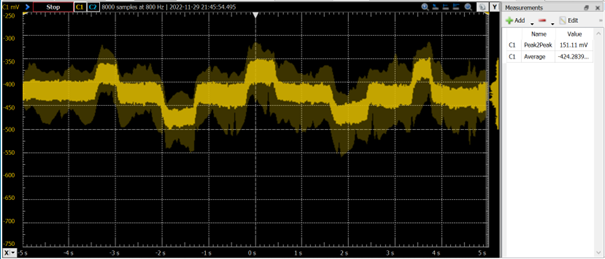
\includegraphics[width=0.9\textwidth]{Fuchs/Messergebnis_RohdatenH.png}
	\caption{Messung der Rohdaten von Augenbewegungen in horizontaler Richtung}
	\label{fig:me_rohdatenH}
\end{figure}

Die zwei obenstehenden Abbildungen \ref{fig:me_rohdatenH} zeigen die Messungen der Rohdaten mit einer Verst"arkung von 51. Bei der Messung der Augenbewegungen in vertikaler Richtung, wie in Abbildung \ref{fig:me_rohdatenV} dargestellt, ist das Blinzeln, welche sich durch steile Amplitudenanstiege kennzeichnet, deutlich zu erkennen. Die maximale Amplitude betr"agt ca. $40-60 mV$. Dividiert man das durch die Verst"arkung, ergibt sich ein Amplitudenwert von $80-110\mu V$. Auff"allig ist der negative Offset von rund $0.667V$.

Invertierender/nicht invertierender

\subsection {AD-Wandlung} \label {adc}

allgemeines

\subsubsection {MCP3208} \label {mcp3208}

Bauteilbeschreibung, Datenblatt!

\subsubsection {Offset} \label{offset}



\subsection {ESP8266} \label {esp}

\textbf{\\Pinout:\\} 
\begin{figure}[h]
	\centering
		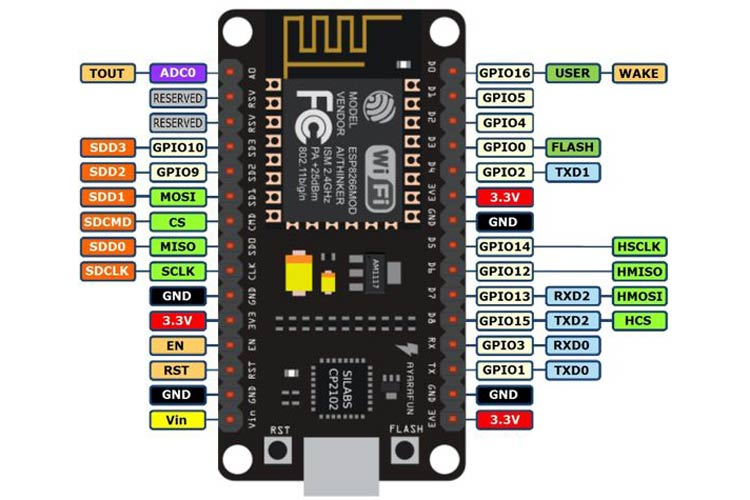
\includegraphics[width=0.9\textwidth]{Alle/ESP8266_Pinout.jpg}
	\caption{Pinout des ESP8266 NodeMCUs}
	\label{fig:esp_pinout}
\end{figure}

Funktionen, Abtastung

\subsection {Analog Discovery} \label{analogdiscovery}

\subsection {Schnittstellen} \label {schnittstellen}

\subsubsection {SPI} \label {spi}

SPI-Schnittstelle allgemein
Pinbelegung, Kommunikation

\subsubsection {Serielle Schnittstelle} \label {serial}

\paragraph {Matlab} \label{matlab}

\subsection {Messergebnisse} \label {messergebnis}



